%%%%%%%%%%%%%%%%%%%%%%%%%%%%%%%%%%%%%%%%%%%%%%%%%%%%%%%%%%%%%%%%%%%%%%
% Lớp 12 | Tọa độ của véc-tơ trong không gian | Véc-tơ và các phép toán véc-tơ trong không gian (chưa tọa độ hóa)
% Dạng 2H2?1-1: Công thức lý thuyết
% Số câu: 24  (sinh tự động bởi tach_cau.py; từ nay thầy sửa trực tiếp file này)
%%%%%%%%%%%%%%%%%%%%%%%%%%%%%%%%%%%%%%%%%%%%%%%%%%%%%%%%%%%%%%%%%%%%%%

%%%%%%%%%%%%%%%% TRẮC NGHIỆM 4 PHƯƠNG ÁN %%%%%%%%%%%%%%%%

% nguồn: Lop_12_Hinh_hoc_Chuong_2
\begin{ex}%[2H2N1-1]%[ma:9ddc7ef6]
	\immini{ 
	Cho hình lập phương $ABCD.A_{1}B_{1}C_{1}D_{1}$. Số đo góc giữa hai véc-tơ $\overrightarrow{AB}$ và $\overrightarrow{A_{1}C_{1}}$ bằng 
	\choice 
		{\True $45^\circ$} 
		{$30^\circ$} 
		{$60^\circ$} 
		{$135^\circ$} 
		 }
		 {
		\begin{tikzpicture}[line join=round,line cap=round,>=stealth,scale=.8,font=\footnotesize]
				\foreach  \x/\y/\z/\g in
					 {
					0/0/B/-135,1.8/1/A/180,4.8/1/D/0,3/0/C/-45, 
					 0/3/B_1/180,1.8/4/A_1/90,4.8/4/D_1/45,3/3/C_1/90
				 }
				\draw (\x,\y) circle  (1pt) coordinate (\z)
					($(\z)+(\g:3.5mm)$) node{$\z$}; 
				\draw[->,dashed,color=black] (A)--(C); 
				\draw[->,color=black]  (A_1)--(C_1);
				 \draw (D_1)--(C_1)--(B_1)--(A_1)--(D_1)--(D)
					 (C_1)--(C)
					 (B_1)--(B)--(C)--(D);
				 \draw[dashed] (A_1)--(A)--(B)
					(A)--(D); 
			\end{tikzpicture}
		 }
	\loigiai{ 
		Ta có $\overrightarrow{A_1C_1} =\overrightarrow{AC}$. Do  đó
		 \[
		\left(\overrightarrow{AB},\overrightarrow{A_1C_1} \right)=\left(\overrightarrow{AB},\overrightarrow{AC}\right)=\widehat{BAC}=45^\circ. 
		 \]
	} 
\end{ex}

% nguồn: Lop_12_Hinh_hoc_Chuong_2
\begin{ex}%[2H2N1-1]%[ma:859e98c7]
	Cho hình bình  hành $ABCD$. Phát biểu nào sau đây~là đúng?
	 \choice
		{$\overrightarrow{AB}+\overrightarrow{AD}=2  \overrightarrow{AC}$}
		{\True  $\overrightarrow{AB}+\overrightarrow{AD}=\overrightarrow{AC}$}
		 {$\overrightarrow{AB}+\overrightarrow{AD}=\overrightarrow{CA}$}
		{$\overrightarrow{AB}+\overrightarrow{AD}=2  \overrightarrow{CA}$}
	 \loigiai{
	 \immini{
		Theo quy tắc hình bình  hành, ta có
		\[\overrightarrow{AB}+\overrightarrow{AD}=\overrightarrow{AC}. \] 
		}{\begin{tikzpicture}[line join=round,line cap=round]
		\def\a{4}; 
		 \def\b{1.5};
		 \def\g{50};
		\path 
			(0,0)  coordinate (D)
			(0:\a) coordinate  (C)
			(\g:\b) coordinate  (A)
			($(A)+(C)-(D)$)  coordinate (B);
		\draw 
			(A)--(B)--(C)--(D)--cycle (A)--(C); 
		\foreach \x/\g in {A/135,B/45,C/-45,D/-135}\fill (\x)  circle (1pt) node[shift={(\g:10pt)}] {$\x$};
	\end{tikzpicture}
		 }
	} 
\end{ex}

% nguồn: Lop_12_Hinh_hoc_Chuong_2
\begin{ex}%[2H2N1-1]%[ma:e0009b91]
	Cho  hình hộp $A B C D. A' B' C' D'$. Phát biểu nào sau đây~là đúng?
	\choice 
		{\True  $\overrightarrow{AB}+\overrightarrow{AD}+\overrightarrow{AA'}=\overrightarrow{AC'}$}
		{$\overrightarrow{AB}+\overrightarrow{AD}+\overrightarrow{AA'}=\overrightarrow{C'A}$} 
		{$\overrightarrow{A B}+\overrightarrow{A D}+\overrightarrow{AA'}=\overrightarrow{AD'}$} 
		 {$\overrightarrow{AB}+\overrightarrow{AD}+\overrightarrow{AA'}=\overrightarrow{D'A}$}
	 \loigiai{
	 \immini{
		Theo  quy tắc hình hộp, ta có
		\[\overrightarrow{AB}+\overrightarrow{AD}+\overrightarrow{AA'}=\overrightarrow{AC'}.  \]
		 }{
		\begin{tikzpicture}[line join=round,line cap=round]
				\def\a{3}; 
				 \def\cao{2};
				 \def\g{30};
				 \path
					(0,0)  coordinate (A)
					(\a,0) coordinate  (B)
					 (\g:{\a/2}) coordinate (D)
					($(B)+(D)-(A)$) coordinate  (C)
					($(A)+(-80:\cao)$) coordinate  (A')
					($(B)+(-80:\cao)$) coordinate  (B')
					($(C)+(-80:\cao)$)  coordinate (C')
					($(D)+(-80:\cao)$) coordinate  (D');
				 \draw
					(A)--(B)--(C)--(D)--cycle  (A')--(B')--(C')
					 (A)--(A')
					 (B)--(B')
					 (C)--(C');
				 \draw[dashed] (A')--(D')--(C')--(A)
					(D)--(D'); 
				 \foreach \x/\g in {A/180,B/-45,C/45,D/90,A'/180,B'/-45,C'/-45,D'/160}\fill (\x) circle (1pt) node[shift={(\g:10pt)}] {$\x$};
				\foreach \x/\y/\z in {}{\draw pic[draw,angle  radius=2mm]{right angle=\x--\y--\z};}
			\end{tikzpicture}
		 }
	} 
\end{ex}

% nguồn: Lop_12_Hinh_hoc_Chuong_2
\begin{ex}%[2H2N1-1]%[ma:79d19b20]
	Trong không gian $Oxyz$, độ dài của vectơ $\vec{u}=(x; y;  z)$ bằng
	\choice{\True $\sqrt{x^2+y^2+  z^2}$}
		{$x^2+y^2+z^2$} 
		{$\sqrt{\dfrac{x^2+y^2+ {z}^2}{3}}$} 
		 {$\dfrac{x^2+y^2+z^2}{3}$}
	\loigiai{ 
		Ta có  $\left|\vec{u}\right|=\sqrt{x^2+y^2+ {z}^2}$.
	} 
\end{ex}

% nguồn: Lop_12_Hinh_hoc_Chuong_2
\begin{ex}%[2H2N1-1]%[ma:c4b766f0]
	 \immini{
	Cho hình hộp $ABCD.A'B'C'D'$. Vectơ  nào dưới đây cùng phương với vectơ $\overrightarrow{AB}$?
	 \choice
		 {$\overrightarrow{C'D}$}
		{$\overrightarrow{AC}$} 
		{\True  $\overrightarrow{CD}$}
		 {$\overrightarrow{B'D'}$}}
		{ 
		\begin{tikzpicture}[scale=.7,line join=round,line cap=round,font=\footnotesize,>=stealth]
				 \def\a{3.5}
				 \def\h{4}
				\path (0:0) coordinate (A) 
					++(0:\a) coordinate  (D)
					++(-130:\a/2) coordinate  (C)
					($(A)+(C)-(D)$) coordinate (B) 
					($(A)!0.25!(C)$) coordinate (H) 
					 ($(H)+(90:\h)$) coordinate (A')
					 ($(A')+(C)-(A)$) coordinate (C')
					($(C')+(B)-(C)$)  coordinate (B')
					($(A')+(D)-(A)$)  coordinate (D');
				\draw[dashed] (B)--(A)--(D) 
					(A)--(A') 
					(A)--(C); 
				\draw (C)--(C')--(D) 
					 (D)--(D')
					 (B)--(B')--(D')
					 (B)--(C)--(D)
					(A')--(B')--(C')--(D')--cycle; 
				\foreach  \x/\g in {A/180,B/180,C/0,D/0,A'/180,B'/180,C'/0,D'/0}
				 \fill (\x) circle (1pt)
					($(\g:4mm)+(\x)$)  node {$\x$};
			\end{tikzpicture}
		} 
	\loigiai{ 
		Hai vectơ $\overrightarrow{AB}$ và $\overrightarrow{CD}$ cùng phương vì  chúng có giá song song với nhau.
	 }
\end{ex}

% nguồn: Lop_12_Hinh_hoc_Chuong_2
\begin{ex}%[2H2N1-1]%[ma:6bf969fc]
	Trong không gian $Oxyz$, côsin của góc giữa hai  vectơ $\vec{u}=(x; y; z)$, \break
	$\vec{u}'=\left(x'; y'; z'\right)$ khác vectơ-không  bằng
	 \choice
		{$\dfrac{xy'+yz'+zx'}{\sqrt{x^2+y^2+z^2}\cdot \sqrt{x'^2+y'^2+z'^2}}$} 
		 {$\dfrac{xz'+yx'+zy'}{\sqrt{x^2+y^2+z^2}\cdot \sqrt{x'^2+y'^2+z'^2}}$}
		 {$\dfrac{xy'+yx'+zz'}{\sqrt{x^2+y^2+z^2}\cdot \sqrt{x'^2+y'^2+z'^2}}$}
		{\True  $\dfrac{xx'+yy'+zz'}{\sqrt{x^2+y^2+z^2}\cdot \sqrt{x'^2+y'^2+z'^2}}$}
	\loigiai{ 
		Ta có  $\cos\left(\vec{u},\vec{u}'\right)=\dfrac{xx'+yy'+zz'}{\sqrt{x^2+y^2+z^2}\cdot \sqrt{x'^2+y'^2+z'^2}}$.
	 }
\end{ex}

% nguồn: Lop_12_Hinh_hoc_Chuong_2
\begin{ex}%[2H2N1-1]%[ma:6ed5d109]
	Phát biểu  nào sau đây~là đúng?
	 \choice
		{$\overrightarrow{AB}-\overrightarrow{AC}=\overrightarrow{BC},\ \forall A, B, C$} 
		{\True $\overrightarrow{AB}-\overrightarrow{AC}=\overrightarrow{CB},\ \forall A, B, C$} 
		{$\overrightarrow{AB}-\overrightarrow{AC}=2 \overrightarrow{BC},\  \forall A, B, C$}
		{$\overrightarrow{AB}-\overrightarrow{AC}=2  \overrightarrow{CB},\ \forall A, B, C$}
	\loigiai{ 
		Theo quy tắc hiệu, ta có $\overrightarrow{AB}-\overrightarrow{AC}=\overrightarrow{CB}$, $\forall  A$, $B$, $C$.
	} 
\end{ex}

% nguồn: Lop_12_Hinh_hoc_Chuong_2
\begin{ex}%[2H2N1-1]%[ma:9a2b5c29]
	Phát biểu nào sau  đây~là đúng?
	 \choice
		{$\overrightarrow{AB}+\overrightarrow{BC}=2 \overrightarrow{AC},\ \forall A,  B, C$}
		 {$\overrightarrow{AB}+2 \overrightarrow{BC}=\overrightarrow{AC},\ \forall A, B, C$}
		{$2  \overrightarrow{AB}+\overrightarrow{BC}=\overrightarrow{AC},\ \forall A, B, C$}
		 {\True $\overrightarrow{AB}+\overrightarrow{BC}=\overrightarrow{AC},\ \forall A, B, C$}
	\loigiai{ 
		Theo  quy tắc 3 điểm, ta có $\overrightarrow{AB}+\overrightarrow{BC}=\overrightarrow{AC}$, $\forall A$, $B$, $C$.
	} 
\end{ex}

% nguồn: Lop_12_Hinh_hoc_Chuong_2
\begin{ex}%[2H2N1-1]%[ma:a98665a6]
	\immini{Cho tứ diện $ABCD$. Gọi $M$ là trung điểm của đoạn thẳng $AB$ (hình bên).  Khi đó vectơ $\overrightarrow{MA}+\overrightarrow{MB}$ bằng
	 \choice
		 {$\overrightarrow{AB}$}
		{\True $\overrightarrow{0}$} 
		 {$\overrightarrow{BA}$}
		 {$2\overrightarrow{MA}$}}
		{ 
		\begin{tikzpicture}
				 \def\a{4}
				 \path (0:0) coordinate (B)
					++(0:\a) coordinate (D) 
					++(-120:\a/2)  coordinate (C)
					($(B)+(70:\a)$) coordinate  (A);
				\path ($(A)!0.5!(B)$)  coordinate (M);
				 \draw[dashed] (B)--(D);
				 \draw (B)--(A)--(D)
					 (A)--(C)
					(B)--(C)--(D); 
				\foreach \x/\g in  {A/90,B/180,C/-45,D/0,M/150}
				\fill  (\x) circle (1.5pt)
					($(\g:3mm)+(\x)$) node  {$\x$};
			\end{tikzpicture}
		 }
	 \loigiai{
		$M$ là trung  điểm của đoạn thẳng $AB$ nên $\overrightarrow{MA}+\overrightarrow{MB}=\overrightarrow{0}$.
	 }
\end{ex}

% nguồn: Lop_12_Hinh_hoc_Chuong_2
\begin{ex}%[2H2N1-1]%[ma:72193ded]
	Trong không gian $Oxyz$, cho hai điểm $A(x;  y; z)$, $B\left(x'; y'; z'\right)$. Tọa độ của vectơ $\overrightarrow{AB}$~là
	 \choice{$\left(x+x'; y+y'; z+z'\right)$}
		 {$\left(x-x'; y-y'; z-z'\right)$}
		{\True  $\left(x'-x; y'-y; z'-z\right)$}
		{$\left(x x'; y y';  z z'\right)$}
	 \loigiai{
		Ta có  $\overrightarrow{AB}=\left(x'-x; y'-y; z'-z\right)$.
	} 
\end{ex}

% nguồn: Lop_12_Hinh_hoc_Chuong_2
\begin{ex}%[2H2N1-1]%[ma:4042d96b]
	Phát biểu nào sau đây~là  đúng?
	 \choice
		{$(a+b) \vec{u}=\vec{u}+b  \vec{u},\ \forall \vec{u}, \forall b \in \mathbb{R}$}
		{$(a+b)  \vec{u}=a \vec{u}+\vec{u},\ \forall \vec{u}, \forall a \in \mathbb{R}$}
		{$(a+b) \vec{u}=a \vec{u}-b \vec{u},\  \forall \vec{u}, \forall a, b \in \mathbb{R}$}
		{\True $(a+b) \vec{u}=a \vec{u}+b \vec{u},\ \forall \vec{u}, \forall  a, b \in \mathbb{R}$}
	 \loigiai{
		Áp dụng tính chất của  phép nhân một số với một véc-tơ, ta có
		\[(a+b) \vec{u}=a \vec{u}+b \vec{u},\ \forall \vec{u}, \forall  a, b \in \mathbb{R}. \]
	 }
\end{ex}

% nguồn: Lop_12_Hinh_hoc_Chuong_2
\begin{ex}%[2H2N1-1]%[ma:bfe22070]
	Trong không gian $Oxyz$, khoảng cách giữa hai điểm $A(x; y; {z})$, $B\left(x'; y'; z'\right)$  bằng
	 \choice{$\sqrt{\left(x'-y\right)^2+\left(y'-x\right)^2+\left(z'-z\right)^2}$}
		 {$\sqrt{\left(x'-z\right)^2+\left(y'-y\right)^2+\left(z'-x\right)^2}$}
		{$\sqrt{\left(x'-x\right)^2+\left(y'-z\right)^2+\left(z'-y\right)^2}$} 
		{\True $\sqrt{\left(x'-x\right)^2+\left(y'-y\right)^2+\left(z'-z\right)^2}$} 
	 \loigiai{
		Ta có  $AB=\sqrt{\left(x'-x\right)^2+\left(y'-y\right)^2+\left(z'-z\right)^2}$.
	 }
\end{ex}

% nguồn: Lop_12_Hinh_hoc_Chuong_2
\begin{ex}%[2H2N1-1]%[ma:da28142d]
	Trong không  gian $Oxyz$, cho hai vectơ $\vec{u}=(x;y;z)$, $\vec{u}'=\left(x';y';z'\right)$. Tọa độ của vectơ $\vec{u}-\vec{u}'$~là
	\choice{$\left(x+x';  y+y'; z+z'\right)$}
		{\True $\left(x-x'; y-y';  z-z'\right)$}
		{$\left(x'-x;  y'-y; z'-z\right)$}
		 {$\left(x x'; y y'; z z'\right)$}
	\loigiai{ 
		Ta có  $\vec{u}-\vec{u}'=\left(x-x'; y-y'; z-z'\right)$.
	 }
\end{ex}

% nguồn: Lop_12_Hinh_hoc_Chuong_2
\begin{ex}%[2H2N1-1]%[ma:b8b12e48]
	Cho  hình hộp $ABCD.A'B'C'D'$. Khi đó $\overrightarrow{BA}+\overrightarrow{BC}+\overrightarrow{BB'}$ bằng
	\begin{center}
		\begin{tikzpicture}[scale=0.8,font=\footnotesize,line join=round,line cap=round,>=stealth]
				\def\a{3} 
				 \def\b{2}
				 \def\h{3.5}
				\path (0:0)  coordinate (A)
					++(0:\a+1)  coordinate (D)
					++(-130:\b) coordinate (C) 
					 ($(A)+(C)-(D)$) coordinate (B)
					($(A)+(85:\h)$)  coordinate (A')
					($(B)+(85:\h)$) coordinate  (B')
					 ($(C)+(85:\h)$) coordinate (C')
					 ($(D)+(85:\h)$) coordinate (D');
				\draw[dashed]  (B)--(A)--(D)
					(A)--(A'); 
				 \draw (C)--(C')
					 (D)--(D')
					(B)--(B') 
					(C)--(C') 
					 (B)--(C)--(D)
					(A')--(B')--(C')--(D')--cycle; 
				\foreach  \x/\g in {A/180,B/180,C/0,D/0,A'/180,B'/180,C'/0,D'/0}
				\fill (\x) circle  (1pt)
					 ($(\g:4mm)+(\x)$) node {$\x$};
			\end{tikzpicture}
	\end{center}
	\choice 
		 {\True $\overrightarrow{BD'}$}
		{$\overrightarrow{BC}$} 
		{$\overrightarrow{BD}$} 
		{$\overrightarrow{BC'}$} 
	 \loigiai{
		Theo quy tắc hình hộp, ta  có $\overrightarrow{BA}+\overrightarrow{BC}+\overrightarrow{BB'}=\overrightarrow{BD'}$.
	} 
\end{ex}

% nguồn: Lop_12_Hinh_hoc_Chuong_2
\begin{ex}%[2H2N1-1]%[ma:e9a0fd10]
	Với mọi véc-tơ $\vec{a}, \vec{b}$, ta  có
	\choice 
		{$\vec{a} \cdot \vec{b}=|\vec{a}|  \cdot|\vec{b}|$}
		{\True $\vec{a}  \cdot \vec{b}=|\vec{a}| \cdot|\vec{b}| \cdot \cos(\vec{a}, \vec{b})$}
		{$\vec{a} \cdot \vec{b}=|\vec{a}| \cdot|\vec{b}|  \cdot \sin(\vec{a}, \vec{b})$}
		{$\vec{a} \cdot  \vec{b}=-|\vec{a}| \cdot|\vec{b}|$}
	\loigiai{ 
		Áp dụng tích vô hướng của  2 véc-tơ, ta có
		\[\vec{a} \cdot \vec{b}=|\vec{a}| \cdot|\vec{b}|  \cdot \cos(\vec{a}, \vec{b}). \]
	 }
\end{ex}

% nguồn: Lop_12_Hinh_hoc_Chuong_2
\begin{ex}%[2H2H1-1]%[ma:ae0f9b9c]
	Trong không gian cho  điểm $O$ và bốn điểm $A$,$B$,$C$,$D$ không thẳng hàng. Điều kiện cần và đủ để $A$,$B$,$C$,$D$ tạo thành hình bình hành là
	 \choice
		{$\overrightarrow{OA}+\dfrac{1}{2}\overrightarrow{OB}=\overrightarrow{OC}+\dfrac{1}{2}\overrightarrow{OD}$} 
		{$\overrightarrow{OA}+\dfrac{1}{2}\overrightarrow{OC}=\overrightarrow{OB}+\dfrac{1}{2}\overrightarrow{OD}$} 
		{\True $\overrightarrow{OA}+\overrightarrow{OC}=\overrightarrow{OB}+\overrightarrow{OD}$}{$\overrightarrow{OA}+\overrightarrow{OB}+\overrightarrow{OC}+\overrightarrow{OD}=\overrightarrow{0}$} 
	\loigiai{ 
		\begin{center}
			\begin{tikzpicture}[scale=1.2]
					\coordinate  [label=above left:$A$] (A) at (0,0);
					\coordinate [label=above right:$B$]  (B) at (3,1);
					\coordinate  [label=below right:$C$] (C) at (5,-1);
					\coordinate [label=below left:$D$] (D) at  (2,-2);
					\fill (A)  circle (1pt);
					\fill  (B) circle (1pt);
					\fill (C) circle  (1pt);
					\fill  (D) circle (1pt);
					 \draw (A) -- (B) -- (C) -- (D) -- cycle;
					\draw[dashed]  (A) -- (C);
					\draw[dashed] (B)  -- (D);
				\end{tikzpicture}
		\end{center}
	Ta có  $$\overrightarrow{OA}+\overrightarrow{OC}=\overrightarrow{OB}+\overrightarrow{OD}\Leftrightarrow \overrightarrow{OA}+\overrightarrow{OA}+\overrightarrow{AC}=\overrightarrow{OA}+\overrightarrow{AB}+\overrightarrow{OA}+\overrightarrow{BC}\Leftrightarrow \overrightarrow{AC}=\overrightarrow{AB}+\overrightarrow{BC}.$$}
\end{ex}

% nguồn: Lop_12_Hinh_hoc_Chuong_2
\begin{ex}%[2H2V1-1]%[ma:c0b46a73]
	 Mệnh đề nào sau đây là \textbf{sai}?
	 \choice
		{$\overrightarrow{a}$, $\overrightarrow{b}$, $\overrightarrow{c}$  đồng phẳng nếu một trong ba vectơ đó bằng $\overrightarrow{0}$}
		{$\overrightarrow{a}$, $\overrightarrow{b}$, $\overrightarrow{c}$ đồng phẳng nếu có  hai trong ba vectơ đó cùng phương}
		{Trong hình hộp $ABCD.A'B'C'D'$ ba vectơ $\overrightarrow{AB'}$, $\overrightarrow{C'A'}$, $\overrightarrow{DA'}$ đồng phẳng} 
		{\True $\overrightarrow{x}=\overrightarrow{a}+\overrightarrow{b}+\overrightarrow{c}$ luôn đồng  phẳng với hai vectơ $\overrightarrow{a}$ và $\overrightarrow{b}$}
	 \loigiai{
		Giả sử cho hình hộp $ABCD.A'B'C'D'$ và gọi $M$ là trung điểm  $C'D'$ khi đó\\
		$\overrightarrow{AB}+\overrightarrow{AD}+\overrightarrow{CM}=\overrightarrow{AM}\Rightarrow\overrightarrow{AM}$ không đồng phẳng với  $\overrightarrow{AB}$, $\overrightarrow{AD}$.
	 }
\end{ex}

% nguồn: Lop_12_Hinh_hoc_Chuong_2
\begin{ex}%[2H2V1-1]%[ma:b6de54aa]
	Cho ba vectơ $\overrightarrow{a}$, $\overrightarrow{b}$, $\overrightarrow{c}$. Điều kiện nào dưới đây khẳng định $\overrightarrow{a}$, $\overrightarrow{b}$,  $\overrightarrow{c}$ đồng phẳng?
	\choice 
		{Tồn tại ba số thực  $m$, $n$, $p$ thỏa mãn $m+n+p=0$ và $m\overrightarrow{a}+n\overrightarrow{b}+p\overrightarrow{c}=\overrightarrow{0}$}
		{\True Tồn tại ba số thực $m$, $n$, $p$ thỏa mãn $m+n+p\ne 0$ và $m\overrightarrow{a}+n\overrightarrow{b}+p\overrightarrow{c}=\overrightarrow{0}$} 
		{Tồn tại ba số thực $m$, $n$,  $p$ sao cho $m\overrightarrow{a}+n\overrightarrow{b}+p\overrightarrow{c}=\overrightarrow{0}$}
		{Giá của $\overrightarrow{a}$, $\overrightarrow{b}$, $\overrightarrow{c}$  đồng qui}
	 \loigiai{
		 Xét $m=n=p=0$ ta luôn có $m+n+p=0$ và $m\overrightarrow{a}+n\overrightarrow{b}+p\overrightarrow{c}=\overrightarrow{0}$ nhưng không thể suy ra
		được $\overrightarrow{a}$,  $\overrightarrow{b}$, $\overrightarrow{c}$ đồng phẳng.\\
		Xét $m+n+p\ne 0$ thì chắc chắn có một trong ba số $m$, $n$, $p$ khác $0$  .\\
		Giả sử $m\ne 0$, suy ra  $m\overrightarrow{a}+n\overrightarrow{b}+p\overrightarrow{c}=\overrightarrow{0}\Leftrightarrow\overrightarrow{a}=-\dfrac{n}{m}\overrightarrow{b}-\dfrac{p}{m}\overrightarrow{c}\Rightarrow\overrightarrow{a}$, $\overrightarrow{b}$, $\overrightarrow{c}$ đồng phẳng.
	} 
\end{ex}

% nguồn: Lop_12_Hinh_hoc_Chuong_2
\begin{ex}%[2H2V1-1]%[ma:01e7de06]
	Cho hình lập phương $ABCD.A'B'C'D'$.  Tính góc giữa hai vectơ $\overrightarrow{BC}$ và $\overrightarrow{B'D'}$.
	\choice 
		{$90^\circ$} 
		 {$60^\circ$}
		 {\True $45^\circ$}
		 {$30^\circ$}
	\loigiai{Ta có $\overrightarrow{B'D'}=\overrightarrow{BD}$  nên $\left(\overrightarrow{B'D'},\overrightarrow{BC}\right)=\left(\overrightarrow{BD},\overrightarrow{BC}\right)=\widehat{DBC}=45^\circ$.}
\end{ex}

% nguồn: Lop_12_Hinh_hoc_Chuong_2
\begin{ex}%[2H2V1-1]%[ma:683a8de7]
	Cho ba véctơ $\overrightarrow{a}$, $\overrightarrow{b}$, $\overrightarrow{c}$ không đồng  phẳng. Khẳng định nào dưới đây đúng?
	 \choice
		{\True $\overrightarrow{x}=\overrightarrow{a}+\overrightarrow{b}+2\overrightarrow{c}$ và $\overrightarrow{y}=2\overrightarrow{a}-3\overrightarrow{b}-6\overrightarrow{c}$ và $\overrightarrow{z}=-\overrightarrow{a}+3\overrightarrow{b}+6\overrightarrow{c}$ đồng  phẳng}
		 {$\overrightarrow{x}=\overrightarrow{a}-2\overrightarrow{b}+4\overrightarrow{c}$ và $\overrightarrow{y}=3\overrightarrow{a}-3\overrightarrow{b}+2\overrightarrow{c}$ và $\overrightarrow{z}=2\overrightarrow{a}-3\overrightarrow{b}-3\overrightarrow{c}$ đồng phẳng}
		{$\overrightarrow{x}=\overrightarrow{a}+\overrightarrow{b}+\overrightarrow{c}$ và $\overrightarrow{y}=2\overrightarrow{a}-3\overrightarrow{b}+\overrightarrow{c}$  và $\overrightarrow{z}=-\overrightarrow{a}+3\overrightarrow{b}+3\overrightarrow{c}$ đồng phẳng}
		{$\overrightarrow{x}=\overrightarrow{a}+\overrightarrow{b}-\overrightarrow{c}$  và $\overrightarrow{y}=2\overrightarrow{a}-\overrightarrow{b}+3\overrightarrow{c}$ và $\overrightarrow{z}=-\overrightarrow{a}-\overrightarrow{b}+2\overrightarrow{c}$ đồng phẳng}
	 \loigiai{
		Ta có $\overrightarrow{x}$, $\overrightarrow{y}$, $\overrightarrow{z}$ đồng  phẳng khi và chỉ khi $\exists m,n:\overrightarrow{x}=m\overrightarrow{y}+n\overrightarrow{z}$ .\\
		Với  $\heva{&\overrightarrow{x}=\overrightarrow{a}+\overrightarrow{b}+2\overrightarrow{c}\\&\overrightarrow{y}=2\overrightarrow{a}-3\overrightarrow{b}-6\overrightarrow{c}\\
		&\overrightarrow{z}=-\overrightarrow{a}+3\overrightarrow{b}+6\overrightarrow{c}}\Rightarrow\overrightarrow{x}=\dfrac{4}{3}\overrightarrow{y}+\dfrac{5}{3}\overrightarrow{z}\Rightarrow\overrightarrow{x}$, $\overrightarrow{y}$,  $\overrightarrow{z}$ đồng phẳng.
	 }
\end{ex}

% nguồn: Lop_12_Hinh_hoc_Chuong_2
\begin{ex}%[2H2V1-1]%[ma:37d20d40]
	 Cho ba véctơ $\overrightarrow{a},\overrightarrow{b},\overrightarrow{c}$ không đồng phẳng. Xét các véctơ $\overrightarrow{x}=2\overrightarrow{a}+\overrightarrow{b}$ và $\overrightarrow{y}=\overrightarrow{a}-\overrightarrow{b}-\overrightarrow{c}$ và $\overrightarrow{z}=-3\overrightarrow{b}-2\overrightarrow{c}$. Khẳng định nào dưới đây là đúng?
	 \choice
		{\True $\overrightarrow{x},\overrightarrow{y},\overrightarrow{z}$ đồng  phẳng}
		 {$\overrightarrow{x},\overrightarrow{a}$ cùng phương}
		 {$\overrightarrow{x},\overrightarrow{b}$ cùng phương}
		{$\overrightarrow{x},\overrightarrow{y},\overrightarrow{z}$ đôi một cùng  phương}
	\loigiai{ 
		Giả sử ba vectơ $\overrightarrow{x},\overrightarrow{y},\overrightarrow{z}$ đồng phẳng khi đó 
		\begin{eqnarray*}
			 &&x=m\overrightarrow{y}+n\overrightarrow{z}\\
			&\Leftrightarrow&  2\overrightarrow{a}+\overrightarrow{b}=m\overrightarrow{a}-\left(m+3n\right)\overrightarrow{b}-\left(m+2n\right)\overrightarrow{c}\\
			&\Leftrightarrow&\heva{&  m=2\\& m+3n=-1\\& m+2n=0}\Leftrightarrow\heva{& m=2\\
			& n=-1.} 
		\end{eqnarray*}
	Vậy $\overrightarrow{x}$, $\overrightarrow{y}$, $\overrightarrow{z}$ đồng phẳng.} 
\end{ex}


%%%%%%%%%%%%%%%% TRẢ LỜI NGẮN %%%%%%%%%%%%%%%%

% nguồn: Lop_12_Hinh_hoc_Chuong_2
\begin{bt}%[2H2V1-1]%[ma:ecedb15b]
	Cho hình chóp $S.ABCD$ có đáy là hình bình hành, mặt bên $SAB$ là tam giác có các  cạnh $AB=5$, $SA=7$, $SB=8$. Tính góc giữa hai véc-tơ $\overrightarrow{C D}$ và $\overrightarrow{S B}$ (đơn vị: độ).
	 \shortans{120}
	\loigiai{ 
	\immini{ 
		Vì $ABCD$ là hình bình hành nên $\overrightarrow{CD}=\overrightarrow{BA}$. Do đó góc giữa hai véc-tơ $\overrightarrow{CD}$ và $\overrightarrow{SB}$ chính là góc giữa 2 véc-tơ $\overrightarrow{BA}$ và $\overrightarrow{SB}$,  chính là góc kề bù với $\widehat{SBA}$.\\
		Áp dụng định lý cô-sin vào tam giác $SAB$, ta có 
		\[\cos \widehat{SBA}=\dfrac{SB^2+AB^2-SA^2}{2SB\cdot AB}=\dfrac{8^2+5^2-7^2}{2\cdot 8\cdot 5}=\dfrac{1}{2}. \] 
		Suy  ra $\widehat{SBA}=60^\circ$.\\
		Vậy góc giữa hai véc-tơ $\overrightarrow{CD}$  và $\overrightarrow{SB}$ bằng
		\[180^\circ-60^\circ=120^\circ. \] 
		}{ 
		\begin{tikzpicture}[>=stealth,line join=round,line cap=round,font=\footnotesize,scale=1]
				\def\a{3.5}; 
				\def\b{2}; 
				 \def\g{30};
				 \def\cao{4};
				\path 
					(0,0) coordinate (A) 
					 (0:\a) coordinate (B)
					 (\g:\b) coordinate (D)
					($(B)+(D)-(A)$) coordinate (C) 
					 (1,\cao) coordinate (S);
				 \draw (S)--(A)--(B)--(C)--(S)--(B);
				\draw[dashed] (A)--(D)--(C) 
					(S)--(D); 
				\foreach  \x/\g in {A/-135,B/-45,C/45,D/150,S/90}\fill (\x) circle (1pt) +(\g:3mm) node {$\x$};
			\end{tikzpicture}
		 }
	 }
\end{bt}


%%%%%%%%%%%%%%%% TỰ LUẬN %%%%%%%%%%%%%%%%

% nguồn: Lop_12_Hinh_hoc_Chuong_2
\begin{bt}%[2H2N1-1]%[ma:3a2a329d]
	Cho hình lăng trụ  $ABC.A'B'C'$.
	\begin{enumerate}
		\item Trong ba vectơ $\overrightarrow{BC}$, $\overrightarrow{CC'}$ và $\overrightarrow{B'B}$ thì vectơ nào bằng vectơ $\overrightarrow{AA'}$? Giải  thích vì sao?
		\item Gọi $M$ là trung điểm của cạnh $BC$. Xác định  điểm $M'$ sao cho $\overrightarrow{MM'}=\overrightarrow{AA'}$.
	\end{enumerate}
	 \loigiai{
		\begin{enumerate}
			\item \immini{Hai đường thẳng $AA'$ và $BC$ chéo nhau nên hai vectơ $\overrightarrow{AA'}$ và  $\overrightarrow{BC}$ không cùng phương.\\
			Do đó, hai vectơ  $\overrightarrow{AA'}$ và $\overrightarrow{BC}$ không bằng nhau.
			Tứ giác $ACC'A'$ là hình bình hành nên $AA'\parallel  CC'$ và $AA'=CC'$.\\
			Hai vectơ $\overrightarrow{AA'}$ và $\overrightarrow{CC'}$ có  cùng độ dài và cùng hướng nên hai vectơ đó bằng nhau.\\
			Tương tự, hai vectơ $\overrightarrow{AA'}$ và $\overrightarrow{B'B}$  có cùng độ dài và ngược hướng nên hai vectơ $\overrightarrow{AA'}$ và $\overrightarrow{B'B}$ không bằng nhau.
			}{ 
			\begin{tikzpicture}[line join=round,line cap=round,font=\footnotesize,scale=1,>=stealth]
					 \def \r{3}
					 \path
						(0,0) coordinate  (A')
						(80:1*\r) coordinate  (A)
						(0:\r) coordinate (C') 
						(-40:0.5*\r) coordinate  (B')
						 ($(A)+(B')$) coordinate (B)
						($(A)+(C')$) coordinate (C) 
						($(B)!0.5!(C)$)  coordinate (M)
						 ($(B')!0.5!(C')$) coordinate (N);
					\draw[-stealth](M)--(N); 
					\draw (A)--(A')--(B')--(C')--(C)--(A)--(B)--(B') 
						(C)--(B); 
					\draw[dashed]  (A')--(C');
					\foreach \x/\g in  {A/90,B/-50,C/90,A'/180,B'/200,C'/0,M/160,N/-80}\fill (\x) circle (1pt)+(\g:.3) node{$\x$};
				\end{tikzpicture}
			 }
			\item Gọi $M'$ là trung điểm của cạnh $B'C'$. Vì tứ giác $BCC'B'$ là hình bình hành nên $MM'\parallel BB'$ và $MM'=BB'$.\\ 
			Hình lăng trụ $ABC.A'B'C'$ có  $AA'\parallel BB'$ và $AA'=BB'$, suy ra $MM'\parallel AA'$ và $MM'=AA'$.\\
			Hai vectơ $\overrightarrow{MM'}$  và $\overrightarrow{AA'}$ có cùng độ dài và cùng hướng nên $\overrightarrow{MM'}=\overrightarrow{AA'}$.\\
			Vậy trung điểm của  cạnh $B'C'$ là điểm $M'$ cần tìm.
		\end{enumerate}
	} 
\end{bt}

% nguồn: Lop_12_Hinh_hoc_Chuong_2
\begin{bt}%[2H2N1-1]%[ma:96138752]
	Cho tứ diện $ABCD$ có độ dài mỗi  cạnh bằng $1$
	\begin{enumerate}
		\item Có bao nhiêu vectơ có điểm đầu là $A$ và  điểm cuối là một trong các đỉnh còn lại của tứ diện.
		\item Trong các vectơ tìm được ở câu a, những vectơ nào có giá nằm trong mặt  phẳng $\left(ABC\right)$.
		\item Tính độ dài của các vectơ tìm được ở  câu a.
	\end{enumerate}
	\loigiai{ 
	\immini{\begin{enumerate}
		\item Có ba vectơ là  $\overrightarrow{AB}$, $\overrightarrow{AC}$ và $\overrightarrow{AD}$.
		 \item Trong ba vectơ $\overrightarrow{AB}$, $\overrightarrow{AC}$ và $\overrightarrow{AD}$ chỉ có hai vectơ là $\overrightarrow{AB}$ và $\overrightarrow{AC}$ có giá nằm trong mặt phẳng $(ABC)$.
		\item Vì tứ diện $ABCD$ có  độ dài mỗi cạnh bằng $1$ nên\\ $\left|AB\right|=\left|AC\right|=\left|AD\right|=1$.
	\end{enumerate}
	 }{
	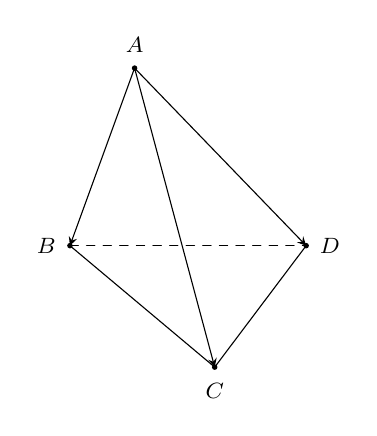
\begin{tikzpicture}[line join=round,line cap=round,font=\footnotesize,scale=1,>=stealth]
			\def \r{3} 
			 \path
				(0,0)  coordinate (B)
				(70:0.8*\r)  coordinate (A)
				(0:\r) coordinate  (D)
				(-40:0.8*\r) coordinate (C); 
			\draw[-stealth](A)--(B); 
			\draw[-stealth](A)--(C); 
			 \draw[-stealth](A)--(D);
			\draw (B)--(C)--(D); 
			\draw[dashed] (B)--(D); 
			\foreach \x/\g in {A/90,B/180,C/-90,D/0}\fill (\x) circle (1pt)+(\g:.3) node{$\x$}; 
		\end{tikzpicture}
	 }
 }
\end{bt}
